\documentclass{article}
\usepackage{geometry}
\geometry{
a4paper,
total={210mm, 297mm},
left=10mm,
right=10mm,
top=30mm,
bottom=20mm,
}

\setlength\parindent{0pt}
\usepackage{hyperref}
\usepackage{graphicx}
\usepackage{subcaption}
\usepackage{amsmath}
\usepackage{mathtools}
\usepackage{amssymb}
\usepackage{lastpage}
\usepackage{parskip}

\begin{document}

{\bf \large 12 March 2015}

The figures below show the results of different experiments on 
v8-FaceDetection44 using Additive BO algorithm.

The experiments on the first row use a guessRange of $7$ to set the
domain of the upperBound.
While the experiments on the second row use a guessRange of $5$.

The figures within the same row use the same experiment parameters except
the initialization points. 

As the guessRange increases and numDiRectEval decreases, 
the model with $d=44$ does not perform as well as models with $d <
44$.

During some experiments, models with $d=8$ or $d=11$ outperform
others.
This agrees with our guess that when optimization becomes difficult
or problem domain becomes large, additive model will have advantages
over the non-additive model.


\begin{figure}[!htbp]
\begin{minipage}{0.45\textwidth}
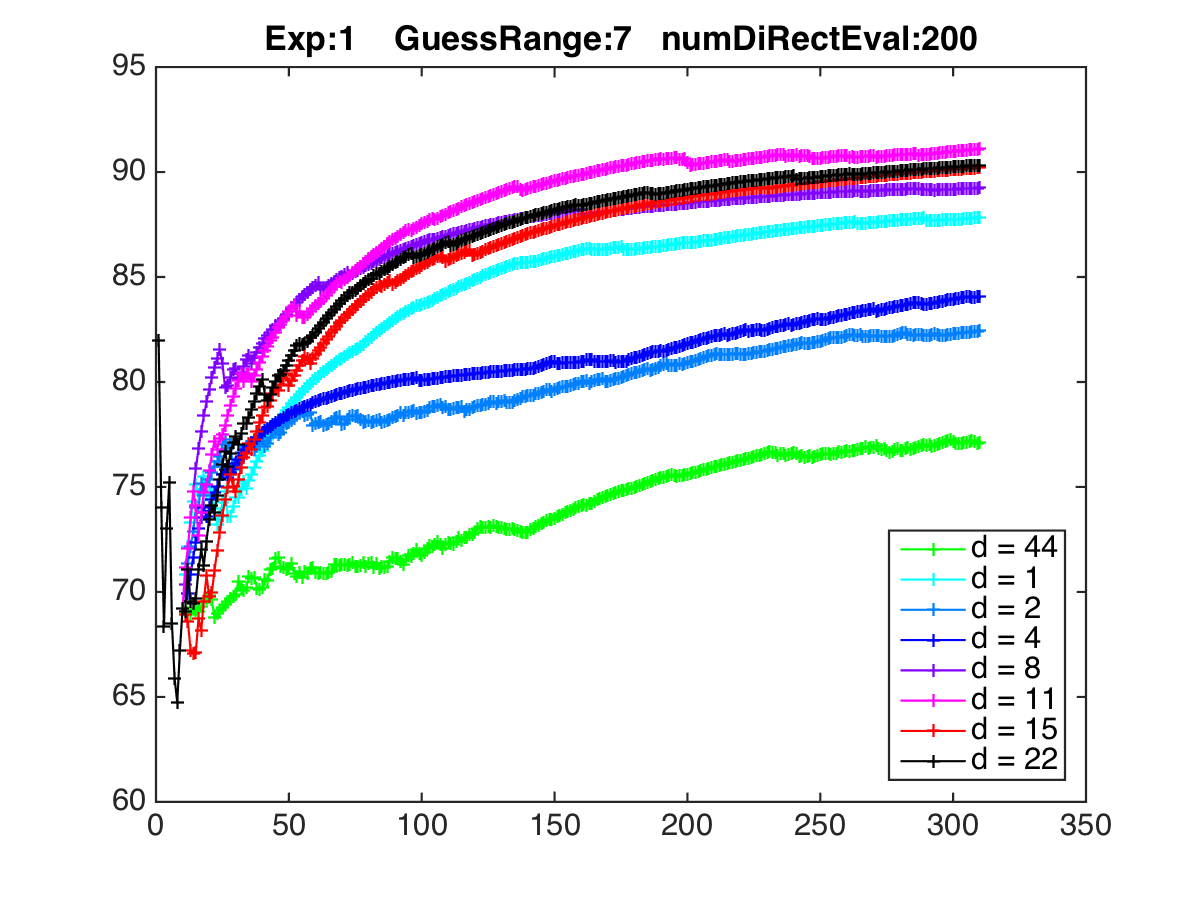
\includegraphics[width = \textwidth]{alpha-1.png}
\end{minipage}
\begin{minipage}{0.45\textwidth}
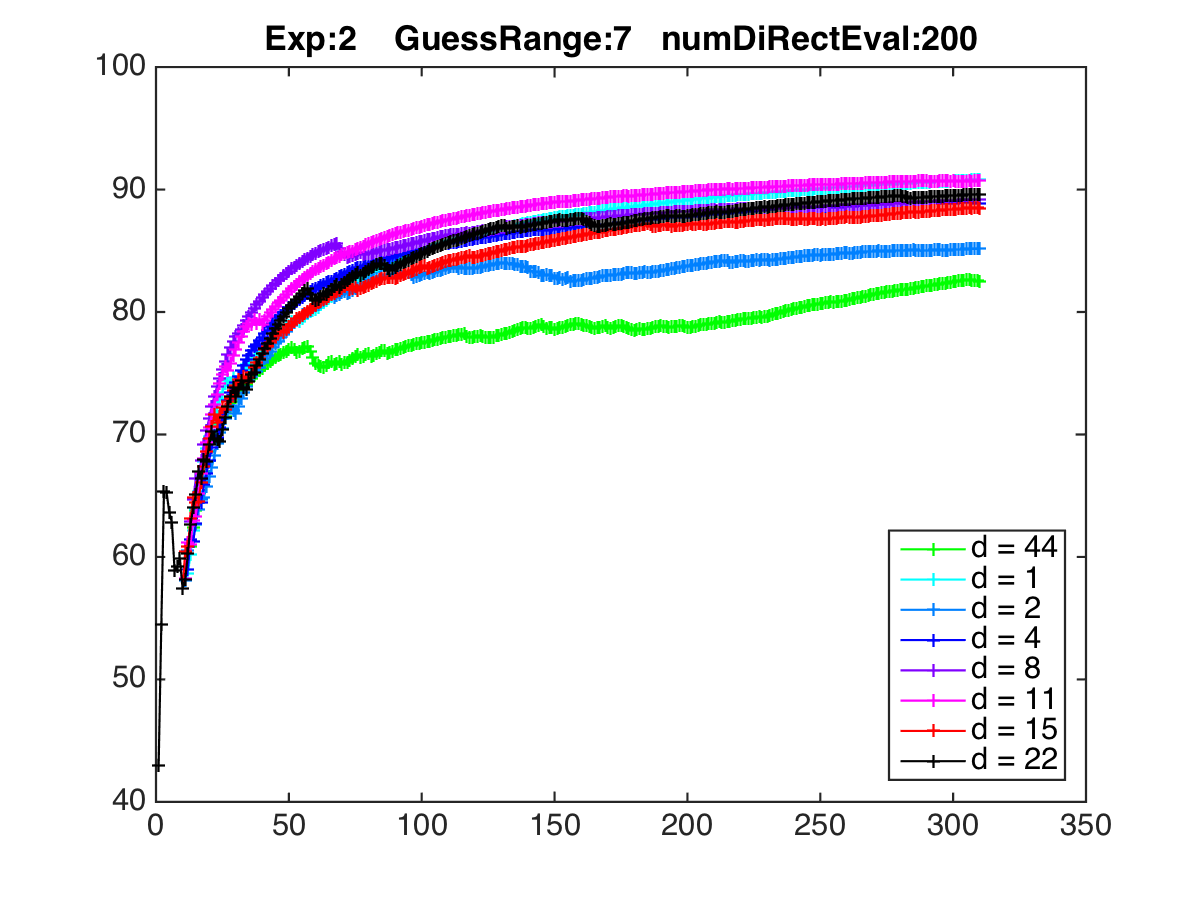
\includegraphics[width = \textwidth]{alpha-2.png}
\end{minipage}
\end{figure}

\begin{figure}[!htbp]
\begin{minipage}{0.45\textwidth}
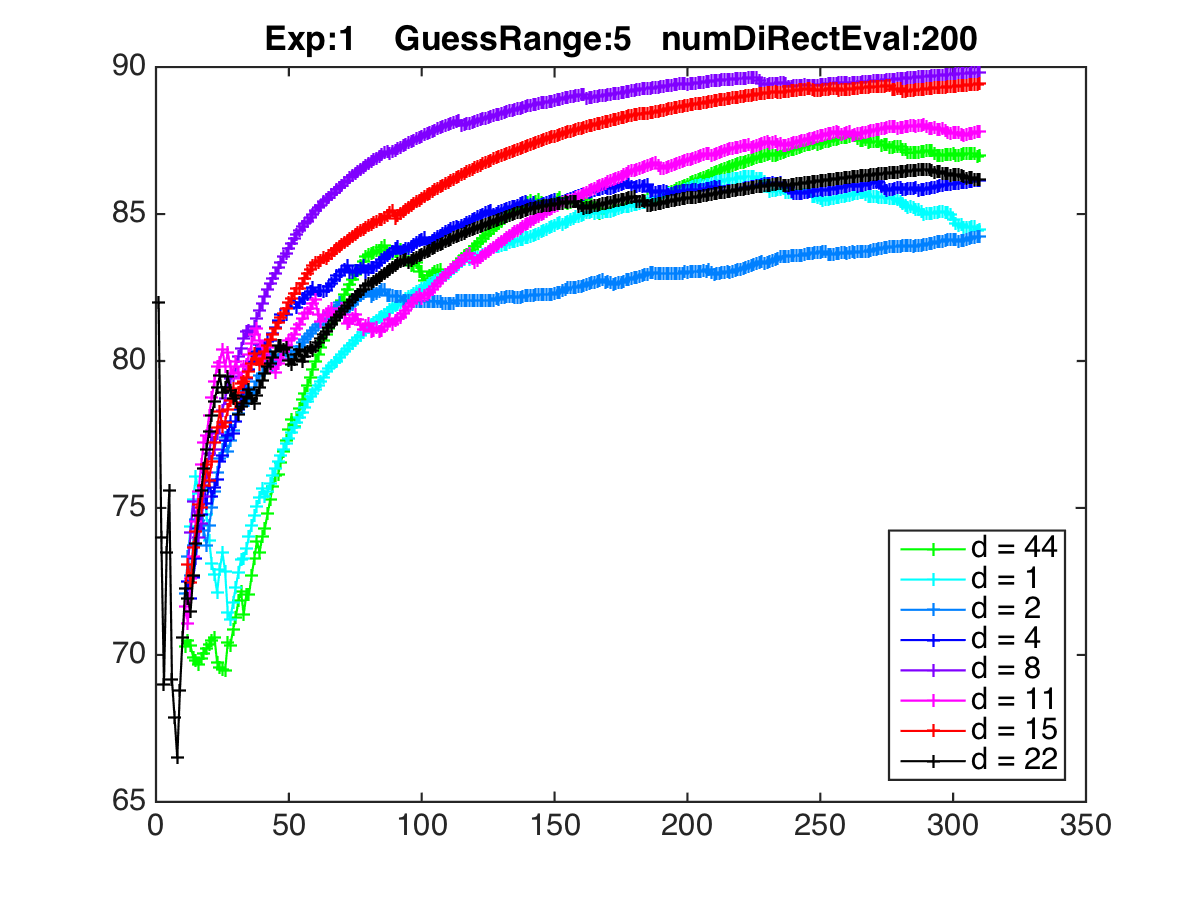
\includegraphics[width = \textwidth]{beta-1.png}
\end{minipage}
\begin{minipage}{0.45\textwidth}
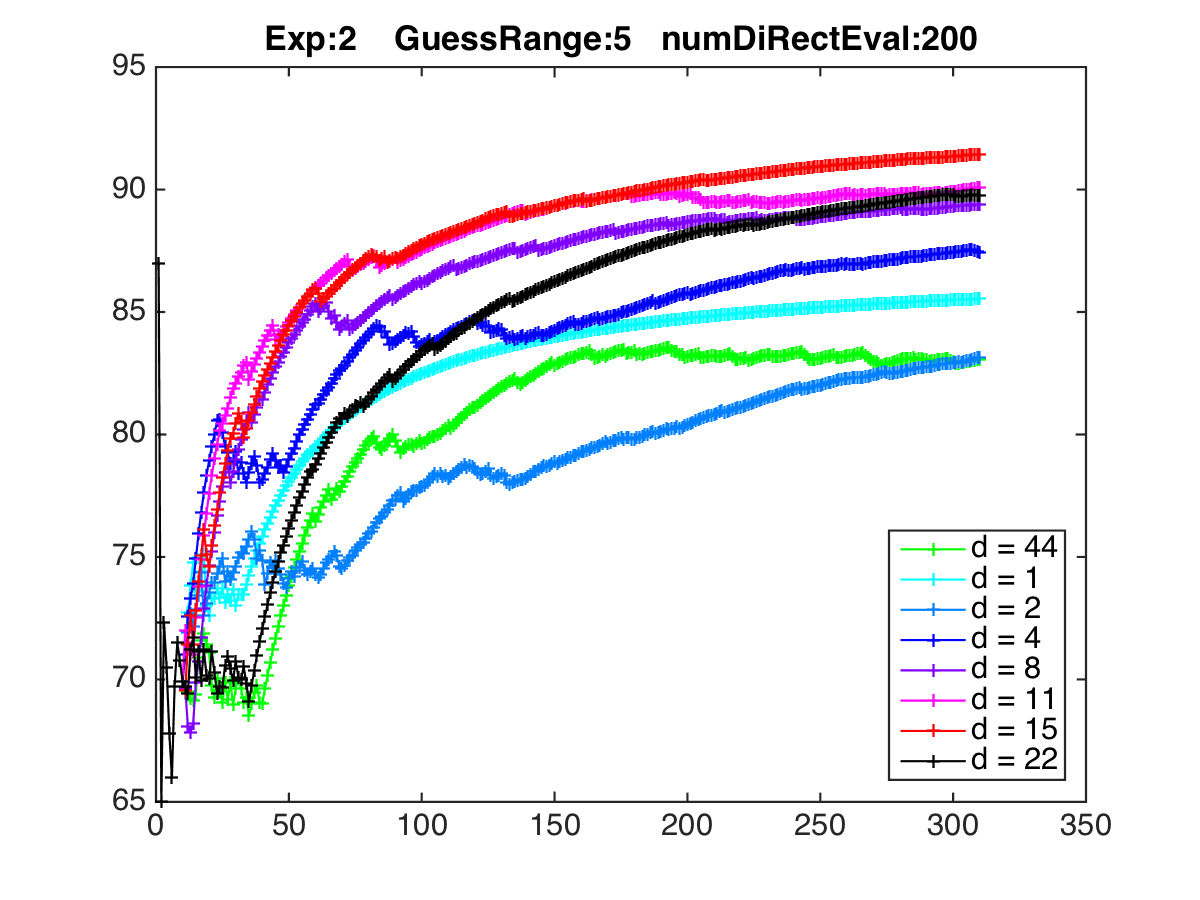
\includegraphics[width = \textwidth]{beta-2.png}
\end{minipage}
\end{figure}


\end{document}
